\documentclass[10pt,twocolumn,letterpaper]{article}

\usepackage{cvpr}
\usepackage{times}
\usepackage{epsfig}
\usepackage{graphicx}
\usepackage{amsmath}
\usepackage{amssymb}
\usepackage{caption}
\usepackage{verbatim}
\usepackage{subcaption}
\usepackage{algorithm2e}
\usepackage{rotating}
\usepackage[space]{grffile}
\usepackage[font=small,skip=0pt]{caption}
%\DeclareMathOperator{\Tr}{Tr}
% Include other packages here, before hyperref.

% If you comment hyperref and then uncomment it, you should delete
% egpaper.aux before re-running latex.  (Or just hit 'q' on the first latex
% run, let it finish, and you should be clear).
\usepackage[breaklinks=true,bookmarks=false]{hyperref}
\graphicspath{ {figures/} }
% \cvprfinalcopy % *** Uncomment this line for the final submission

\def\cvprPaperID{2349} % *** Enter the CVPR Paper ID here
\def\httilde{\mbox{\tt\raisebox{-.5ex}{\symbol{126}}}}

% custom commands
\newcommand{\scream}[1]{{\color{red} \bf *** #1 ***}}

% Pages are numbered in submission mode, and unnumbered in camera-ready
%\ifcvprfinal\pagestyle{empty}\fi
\setcounter{page}{1}
\begin{document}

%%%%%%%%% TITLE
\title{Supplementary Material for the Paper ``Enriching Object Detection with\\2D-3D Registration and Continuous Viewpoint Estimation''}
%\title{Enrich Object Detection : 2D-3D registration and continuous viewpoint estimation}

% \author{First Author\\
% Institution1\\
% Institution1 address\\
% {\tt\small firstauthor@i1.org}
% % For a paper whose authors are all at the same institution,
% % omit the following lines up until the closing ``}''.
% % Additional authors and addresses can be added with ``\and'',
% % just like the second author.
% % To save space, use either the email address or home page, not both
% \and
% Second Author\\
% Institution2\\
% First line of institution2 address\\
% {\tt\small secondauthor@i2.org}
% }

\maketitle
%\thispagestyle{empty}

%%%%%%%%% BODY TEXT
We present qualitative results in the supplementary material for our paper ``Enriching Object Detection with 2D-3D Registration and Continuous Viewpoint Estimation''.
% In Sect.~\ref{sec:3dobject}, we present detection result on qualitative results.

\section{3D Object Dataset}
\label{sect:3dobject}
We run our ensemble of NZ-WHO templates as a detector on 3D Object dataset\cite{savarese07} and present detection average precision, average viewpoint precision, viewpoint confusion matrix and mean precision in pose estimation. See Fig.~\ref{fig:3dobject_ap}

\begin{figure}[h]
  \centering
  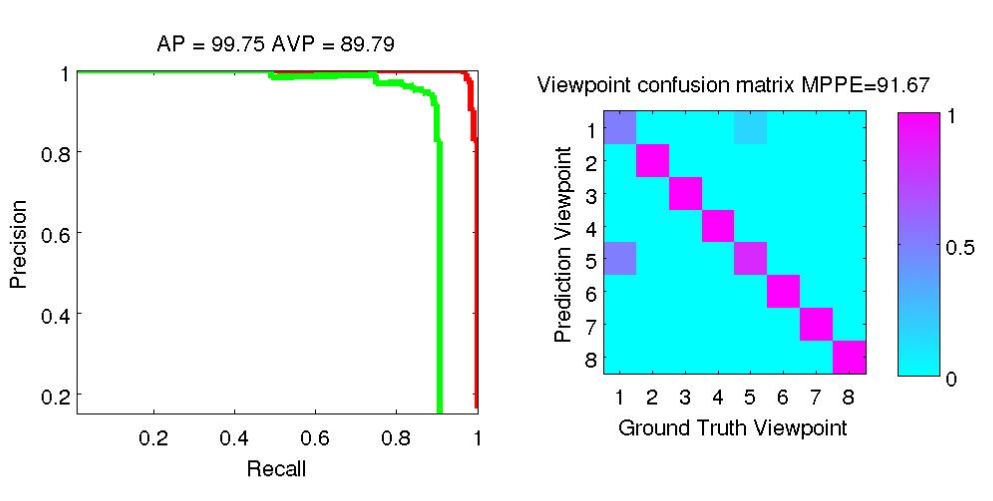
\includegraphics[width=0.99\linewidth]{supp/car_ap_3dobject_tight.png}\\
  \vspace{-5pt}
  (a) Car\\
  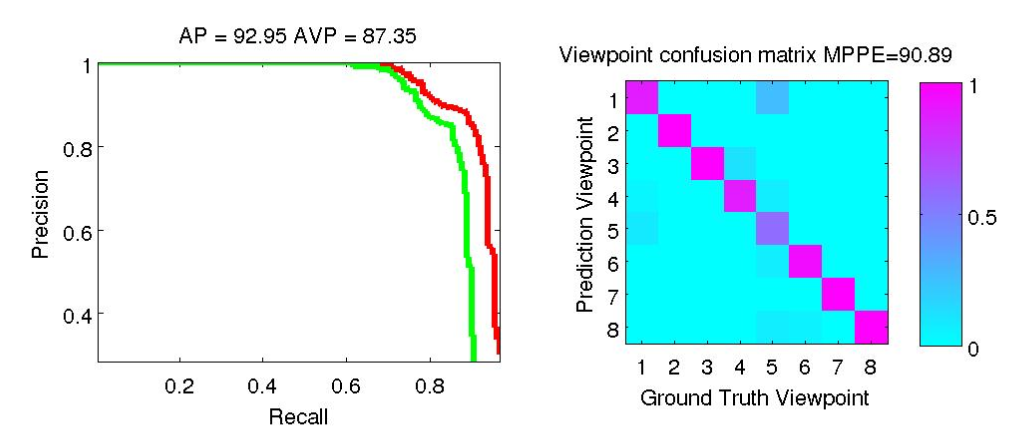
\includegraphics[width=0.99\linewidth]{supp/bicycle_ap_3dobject_tight.png}\\
  \vspace{-5pt}
  (b) Bicycle
\caption{Detection and pose estimation on 3D Object dataset car category. (left) Average Precision (AP) and Average Viewpoint Precision (AVP) and (right) Viewpoint confusion table and MPPE, Viewpoint index 1 is front, 2 is front-right, 5 is back and 8 is front-left. Most of the error in viewpoint estimation come from frontal and back views}% with a bounding box and corresponding confidence score (right).}
  \label{fig:3dobject_ap}
\end{figure}

More qualitative results are on the Fig.~\ref{fig:3dobject_fig}. The each of the template in the ensemble of NZ-WHO templates has a corresponding rendering and a CAD model. These can be transferred as a metadata and overlay the rendering on top of the detection.

\begin{figure*}[h]
\setlength\tabcolsep{1pt}
\centering
\begin{tabular}{|c|c|}
  \hline
  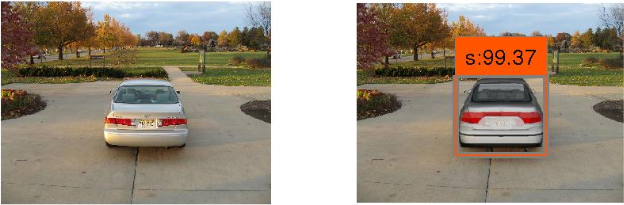
\includegraphics[width=0.40\linewidth]{supp/car1.png} &
  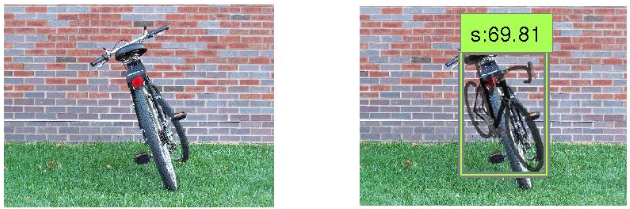
\includegraphics[width=0.40\linewidth]{supp/bicycle1.png} \\
  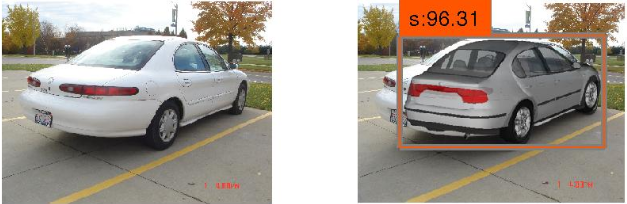
\includegraphics[width=0.40\linewidth]{supp/car23.png} &
  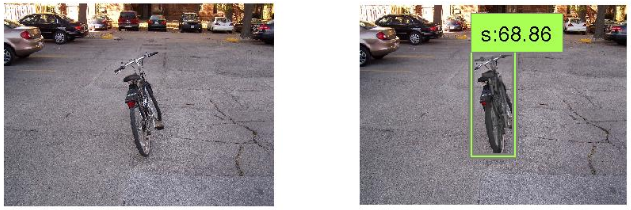
\includegraphics[width=0.40\linewidth]{supp/bicycle3.png} \\
  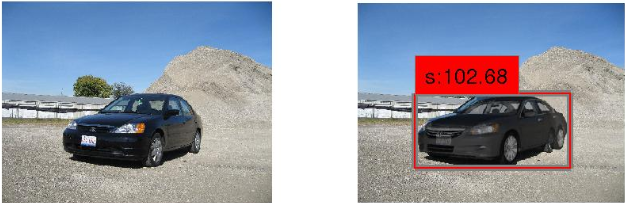
\includegraphics[width=0.40\linewidth]{supp/car26.png} &
  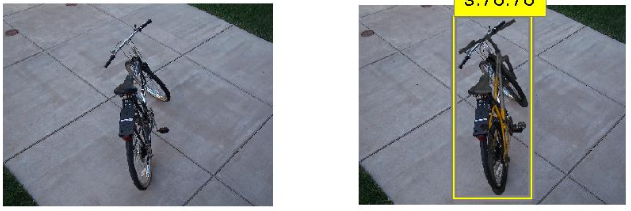
\includegraphics[width=0.40\linewidth]{supp/bicycle4.png} \\
  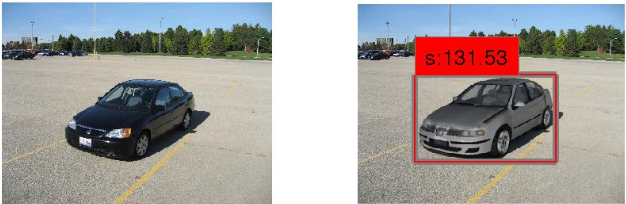
\includegraphics[width=0.40\linewidth]{supp/car29.png} & 
  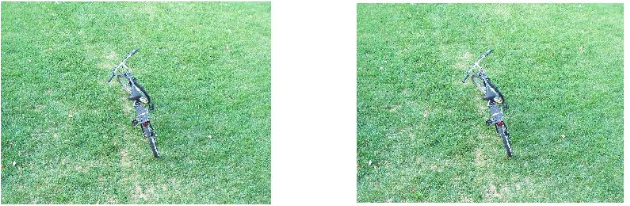
\includegraphics[width=0.40\linewidth]{supp/bicycle5.png} \\
  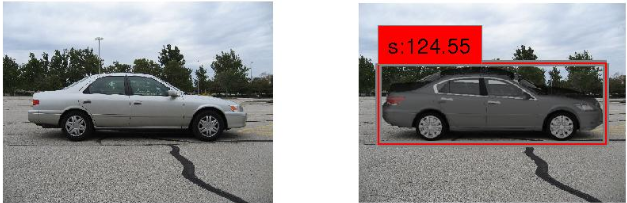
\includegraphics[width=0.40\linewidth]{supp/car10.png} &
  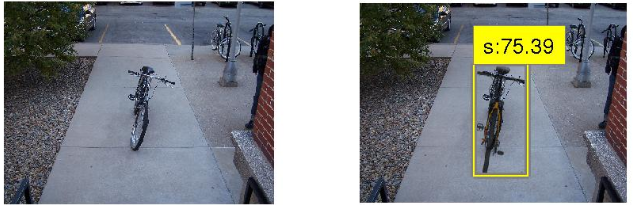
\includegraphics[width=0.40\linewidth]{supp/bicycle9.png} \\
  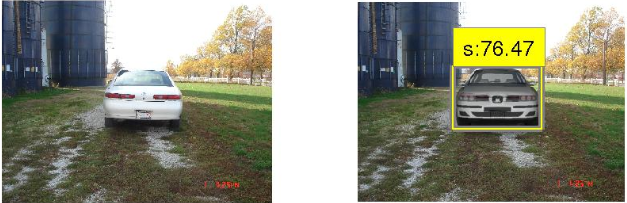
\includegraphics[width=0.40\linewidth]{supp/car13.png} &
  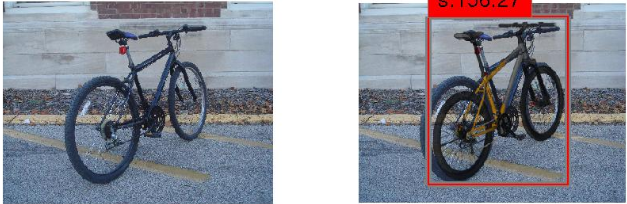
\includegraphics[width=0.40\linewidth]{supp/bicycle13.png} \\
  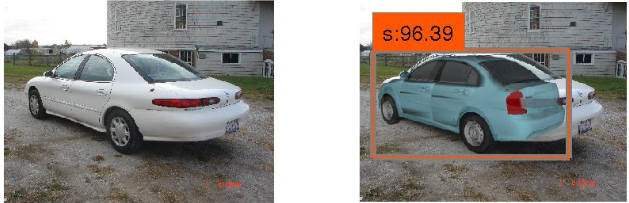
\includegraphics[width=0.40\linewidth]{supp/car15.png} &
  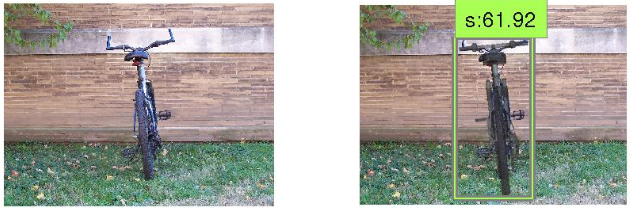
\includegraphics[width=0.40\linewidth]{supp/bicycle11.png} \\
  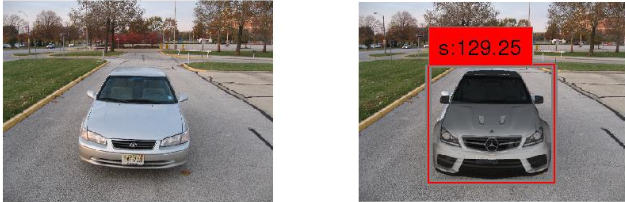
\includegraphics[width=0.40\linewidth]{supp/car8.png} &
  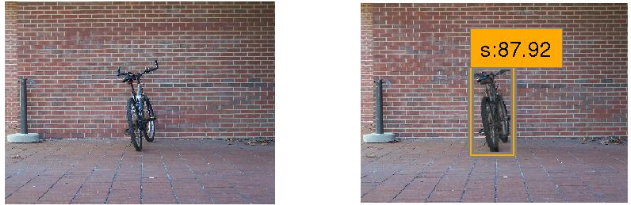
\includegraphics[width=0.40\linewidth]{supp/bicycle12.png} \\
  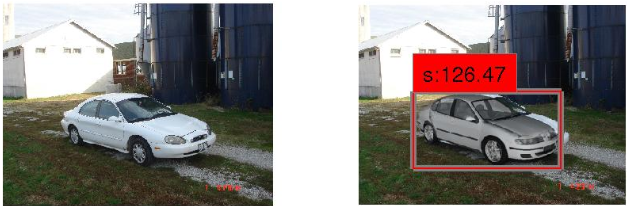
\includegraphics[width=0.40\linewidth]{supp/car20.png} & 
  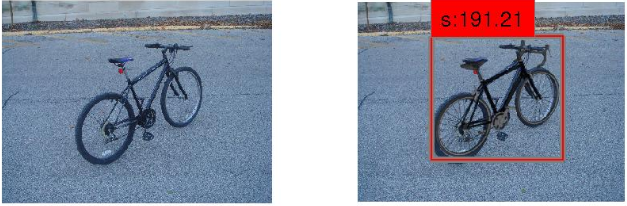
\includegraphics[width=0.40\linewidth]{supp/bicycle15.png} \\
  \hline
  Car & Bicycle \\
  \hline
  \end{tabular}
\caption{Detection results on 3D Object dataset car and bike classes. In each column, original image (left) and detection result overlaid on top (right).}% with a bounding box and corresponding confidence score (right).}
  \label{fig:3dobject_fig}
\end{figure*}

\clearpage
\clearpage
{\small
\bibliographystyle{ieee}
\bibliography{egbib}
}

\end{document}
